\section{Questão 1}

A base de dados apresentada foi recriada recorrendo á aplicação MySQLWorkbench\cite{ref_intro} e foi povoada utilizando o seguinte script:

\begin{figure}[H]

  \centering
  \captionsetup{justification=centering}

  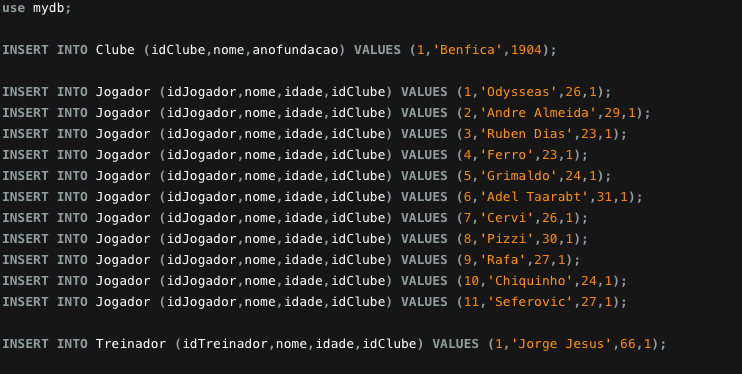
\includegraphics[width = 0.8\textwidth]{povoamento1.png}
  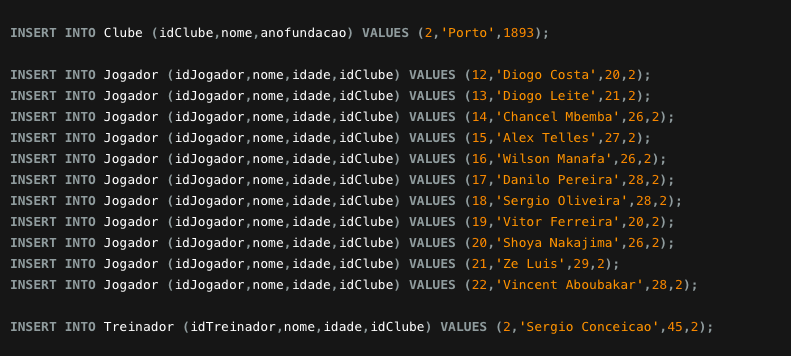
\includegraphics[width = 0.8\textwidth]{povoamento2.png}
  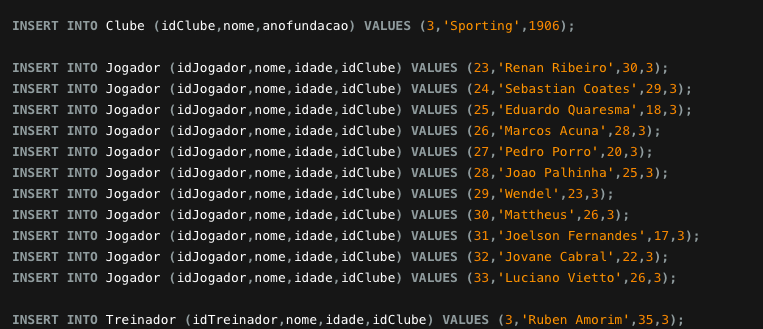
\includegraphics[width = 0.8\textwidth]{povoamento3.png}
  
  \caption {Script utilizado para realizar o povoamento da base de dados}

  \label{fig:povoamento}
\end{figure}


O povoamento da mesma pode ser confirmado realizando uma consulta á base de dados em questão como se mostra na figura abaixo:

\begin{figure}[H]

  \centering
  \captionsetup{justification=centering}

  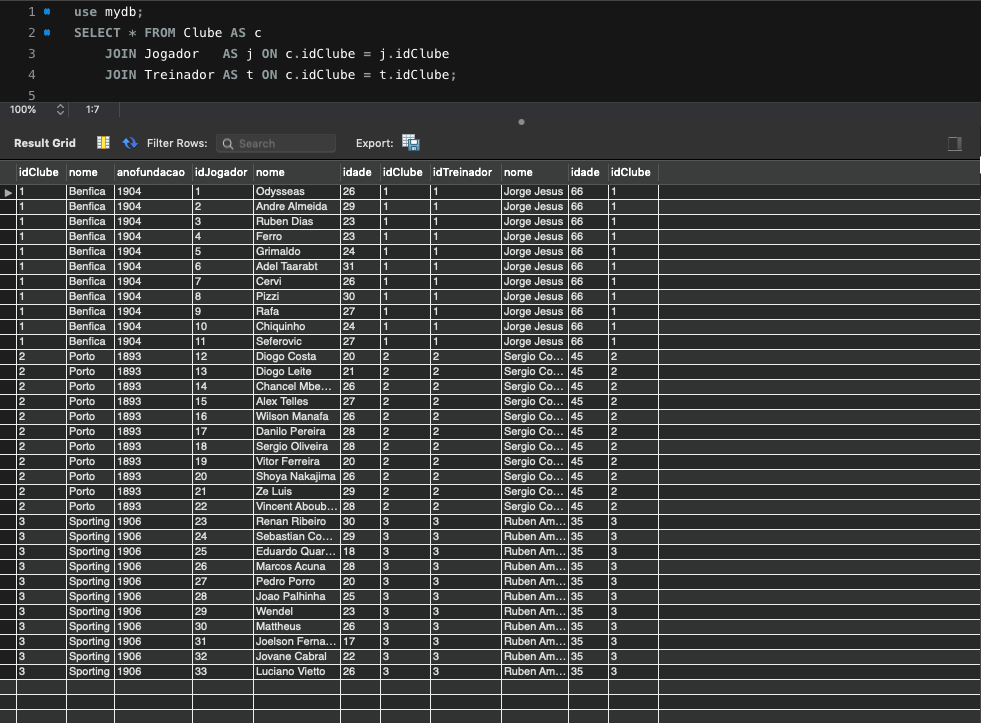
\includegraphics[width = 0.8\textwidth]{prova1.png}
  
  \caption {Visualização da base de dados povoada}

  \label{fig:baseDeDados}
\end{figure}
